\chapter{Project Implementation}
Initiating the chapter, here project implementation is discussed. The resources required, flowcharts, algorithms as well as proposed layouts have been highlighted here.
\section{Requirement of Resources}
\begin{itemize}
    \item Software Requirement 
        \begin{enumerate}
            \item OS Requirement:
                \begin{itemize}
                    \item Windows 8/10(Can be used both for Training and at User End)
                    \item Linux(Only at User End)
                \end{itemize}
            \item Training of the model:
                \begin{itemize}
                    \item Python ide(Anaconda Jupyter Notebook/Jupyter Lab)
                    \item Dataset for Training
                \end{itemize} 
            \item Web Application
        \end{enumerate}
    \item Hardware Requirement
        \begin{enumerate}
            \item Basic Hardware for Training Purpose:
                \begin{itemize}
                    \item RAM : 8 GB
                    \item ROM : 2 GB
                    \item Processor : i5 Processor
                \end{itemize}
        \end{enumerate}
    \end{itemize}



%%%%%%%%%%%%%%%%%%%%%%%%%%%%%%%%%%%%%%%%%%%%%%%%%%%%%%%%%%%%%%%%%%%%%%%%%%%%%%%%%%%%%%%%%%%%%%%%%%%%%%%%%%%%%%%%%%%%%%%%%%%%%%%%%%%%%%%%%%%%%%%%%%%%%%%%%%%%%%%%%%%%%%%%%%%%%%%%%%%%%%%%%%%%%%%%%%%%%%%%%%%%%%%%%%%%%%%%%%%%%%%%%%%%%%%%%%%%%

\section{Development of the Detection model}
This section explains about the Detection model and it's training. The model developed is the backend of this project, as it handles the core function of determining whether the MRI image present has tumour or not.
\subsection{Algorithm}
Step 1 : Import the libraries.\\ 
Step 2 : Import the datasets.\\ 
Step 3 : Create the root directory to store the Final Dataset.\\ 
Step 4 : Create the sub directories to store the images based on tumour presence/absence.\\ 
Step 5 : Augment the dataset.
Step 6 : Copy tumorous images from datasets into the Yes subdirectory.\\ 
Step 7 : Copy non-tumorous images from datasets into the No subdirectory.\\
Step 8 : One Hot Encode the images.\\ 
Step 9 : Creating data list for storing image data in numpy form, path list for storing paths of all images and result list to store data of Step 7.\\ 
Step 10 : Splitting data into train, test, and validation.\\ 
Step 11 : Defining Model Layers.\\ 
Step 12 : Defining Callbacks.\\ 
Step 13 : Training the Model.\\ 
Step 14 : Plotting the accuracy and loss graphs.\\ 
Step 15 : Evaluating the Model.\\ 
Step 16 : Manually testing the model with user input.\\ 
\subsection{Flowchart}
The flowchart below describes the process as to how the detection model is developed.
\begin{figure}[H]
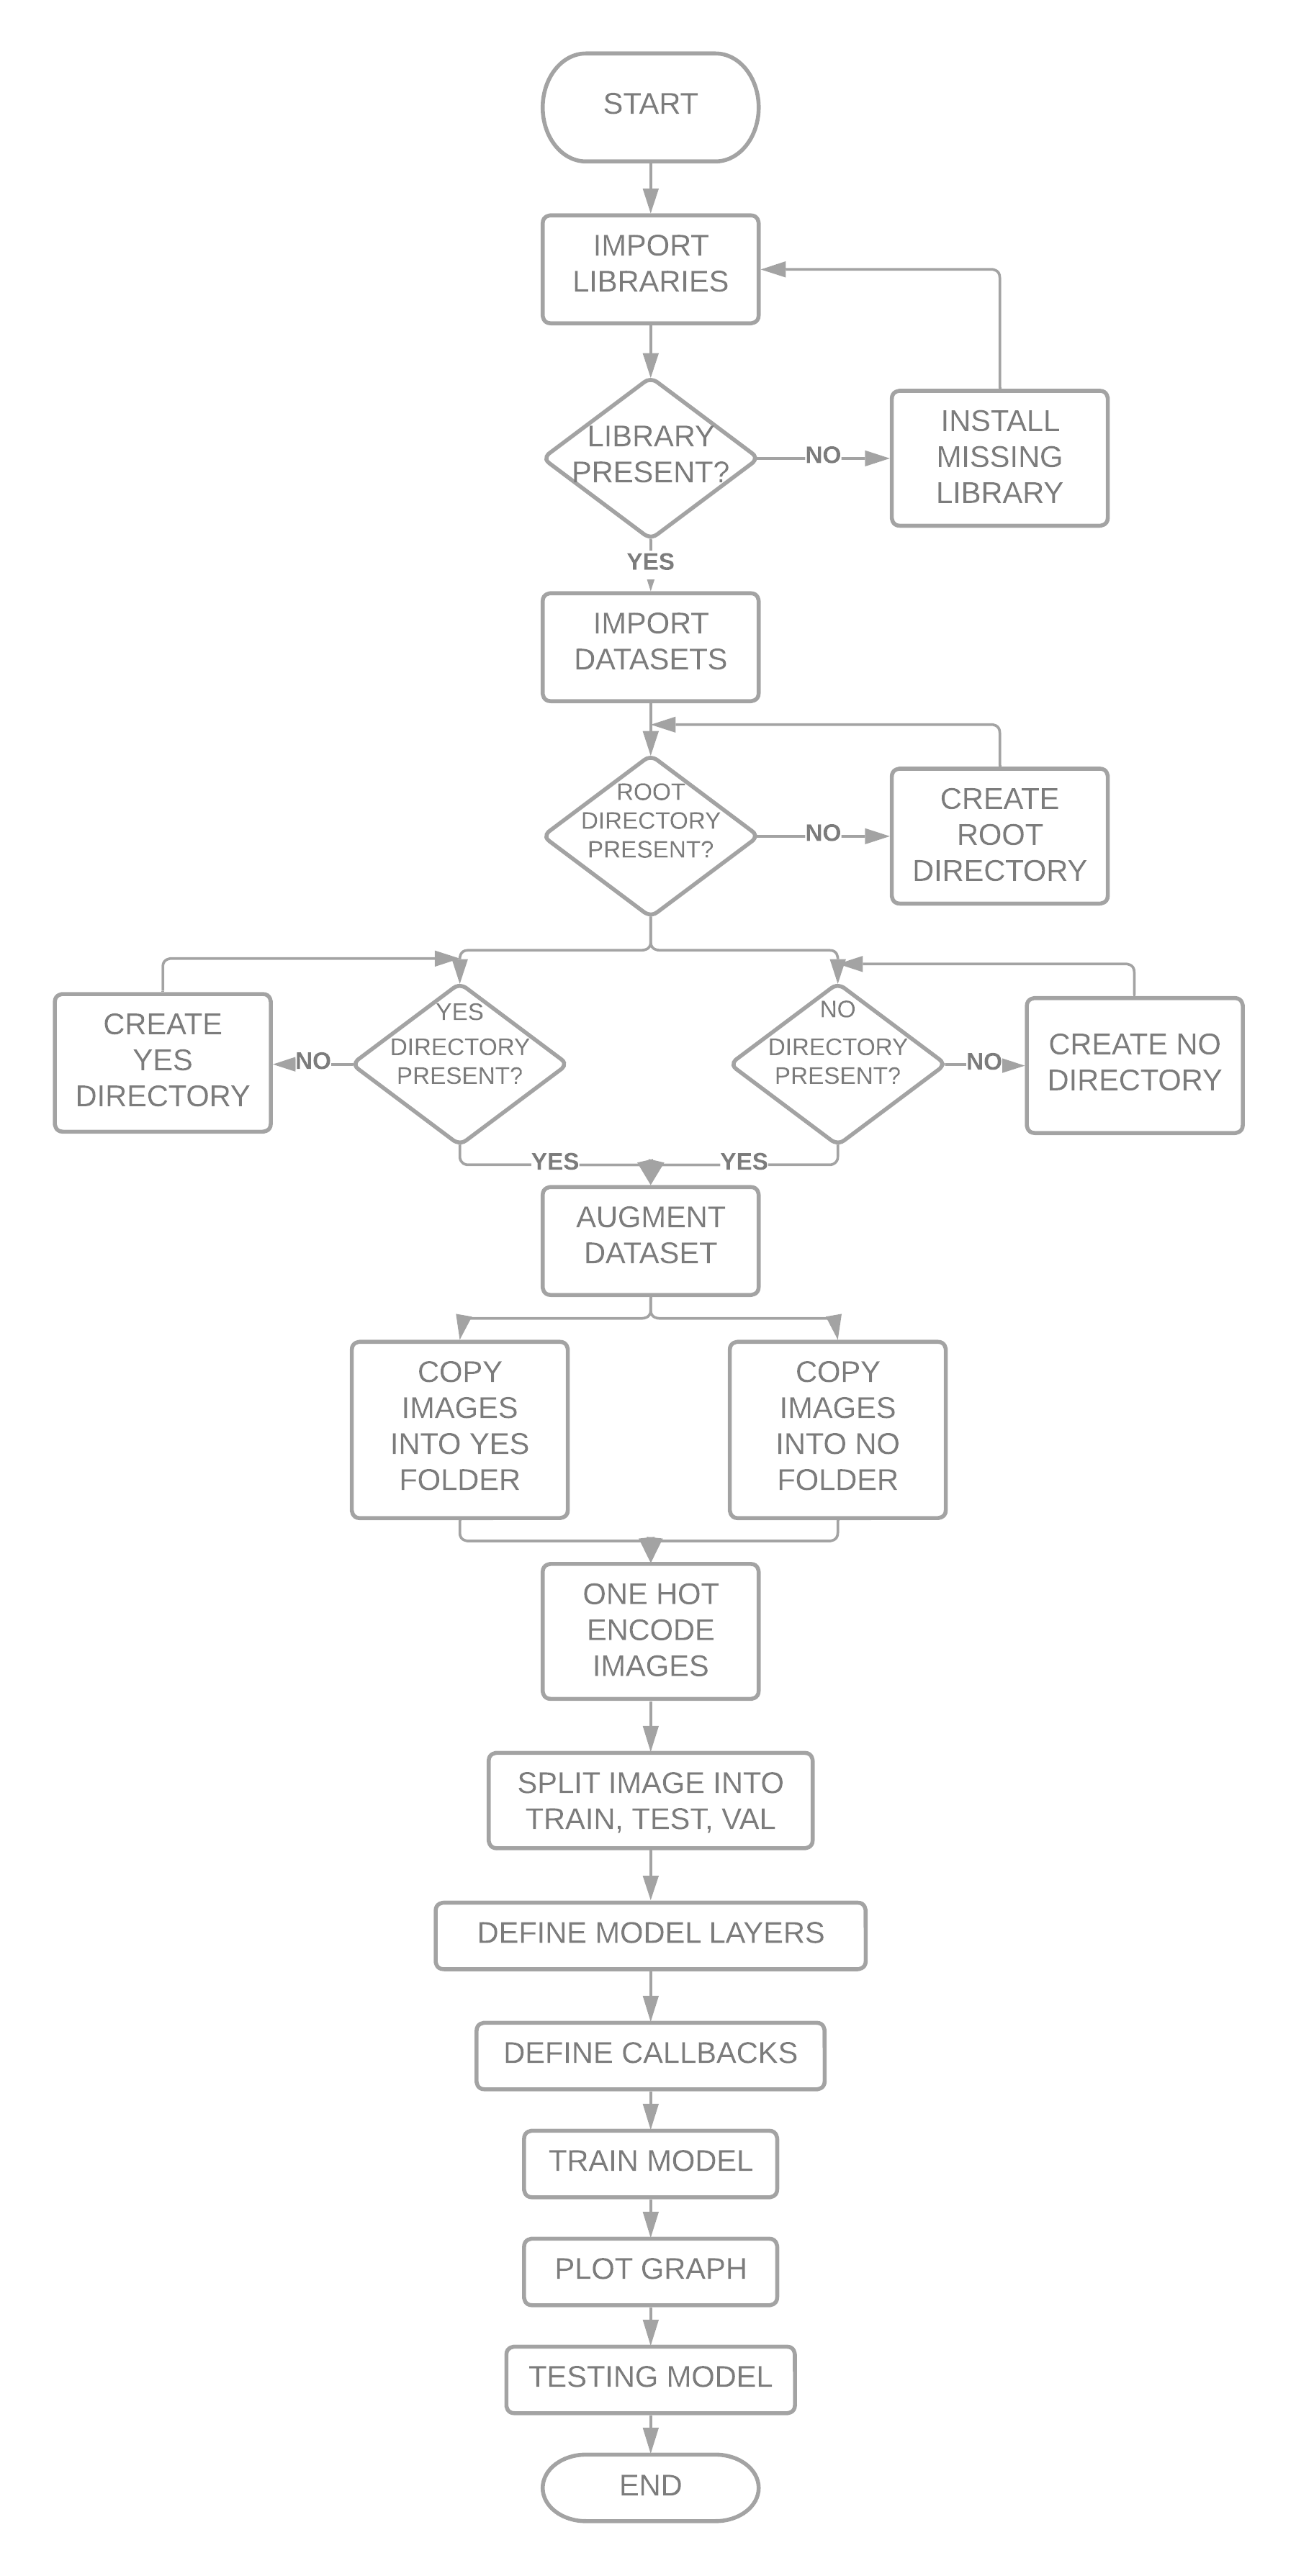
\includegraphics[scale=0.18]{Photos/model_flowchart.png}
\caption{Model Training Flowchart} \label{fig:model_flowchart}
\end{figure}
\subsection{Image Augmentation}
Image Augmentation is a technique that can be used to artificially expand the size of a training set by creating modified data from the existing one. It is a good practice to use DA if you want to prevent overfitting, or the initial dataset is too small to train on, or even if you want to squeeze better performance from your model. Figure \ref{fig:ImageAugmentation} shows an output to an image that has been augmented.
\begin{figure}[H]
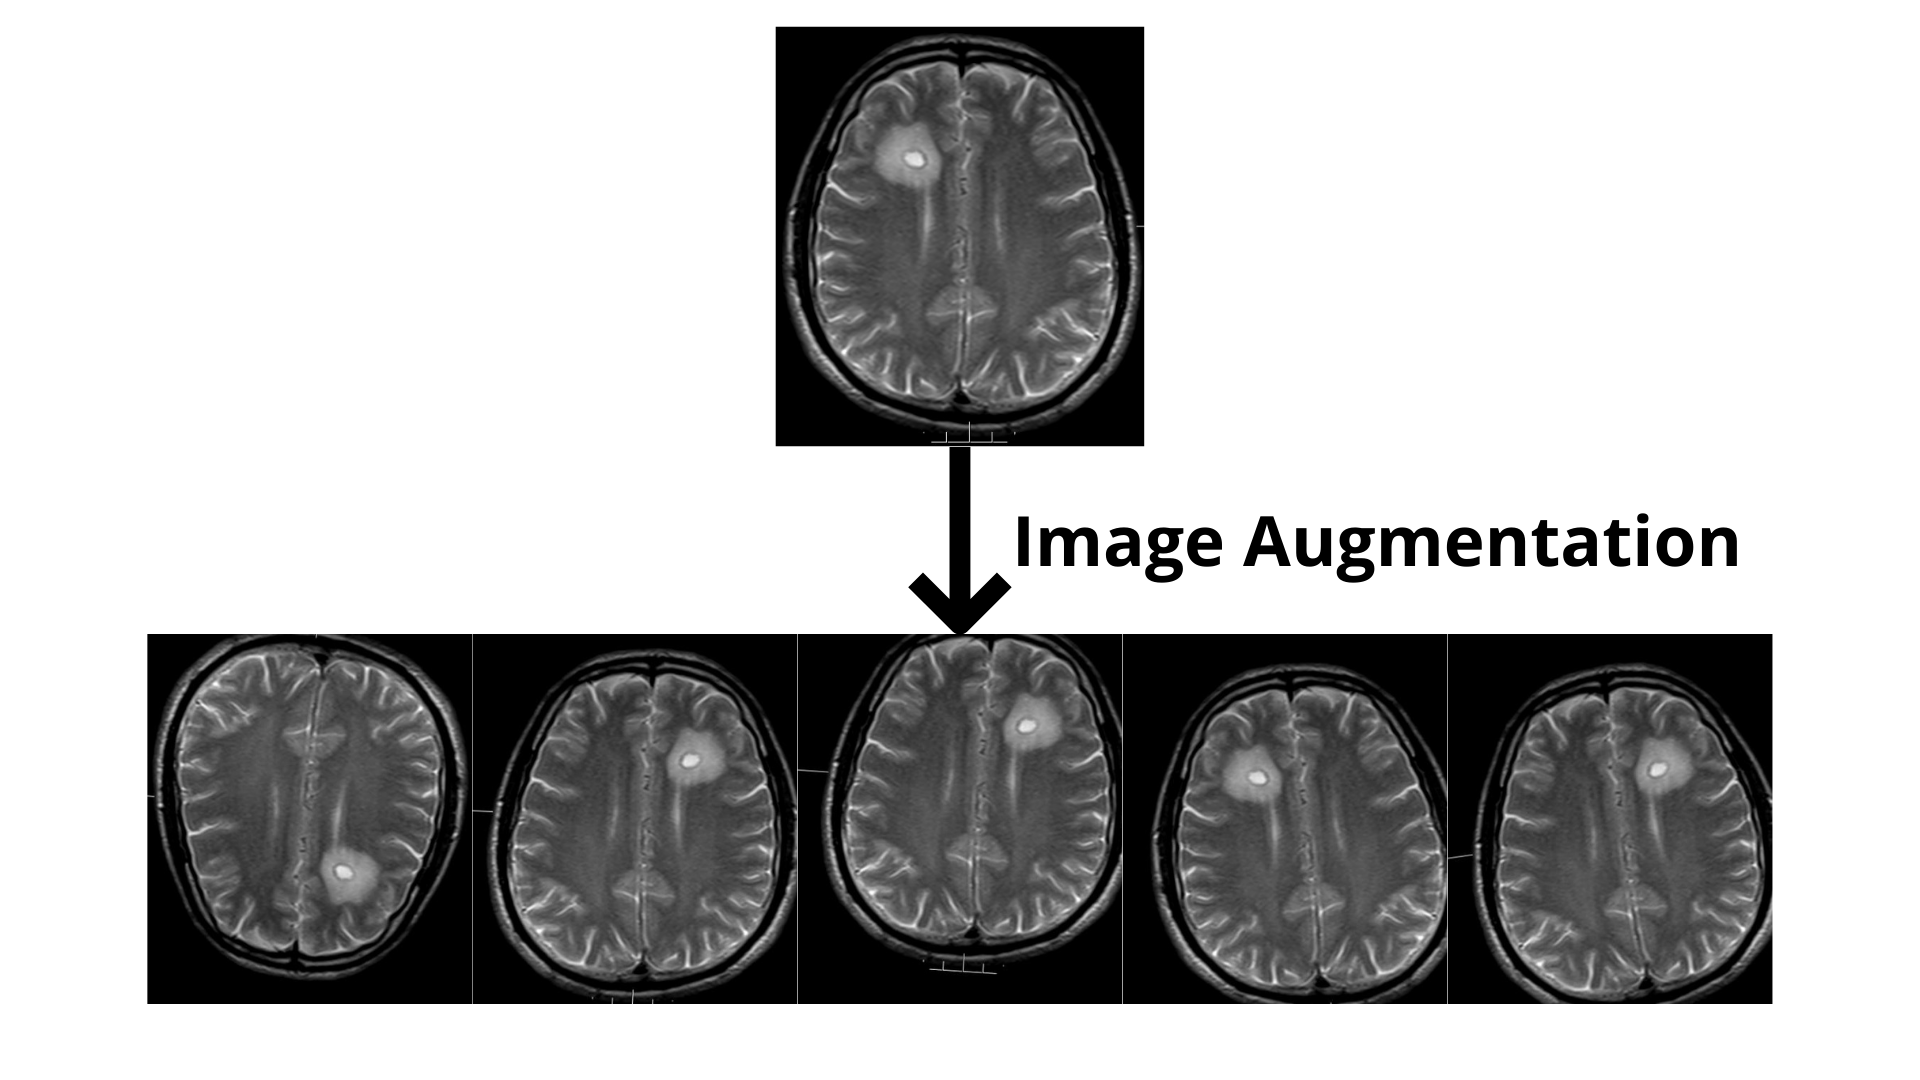
\includegraphics[scale=0.18]{Photos/ImageAugmentation.png}
\caption{Image Augmentation} \label{fig:ImageAugmentation}
\end{figure}
\subsection{Defining the Model}
The figure below summarises the model layers. A sequential model was used for the project. It is the easiest way to build a model in Keras. It allows you to build a model layer by layer. Each layer has weights that correspond to the layer the follows it.Figure \ref{fig:model_plot} shows the model architecture used in the development of the model. We use the 'add()' function to add layers to the model. To define the model following libraries must be imported, these libraries are a sub class of "keras.layers" :
\begin{itemize}
    \item Sequential : It is used to initialize the neural network.
    \item Convolution2D : This layer deals with creating a convolutional network that will deal with the MRI images.
    \item MaxPooling2D : This layer adds the pooling layers.
    \item Flatten : This layer converts the pooled feature map to a single column. This is passed to the fully connected layer.
    \item Dense : Dense layer will add this fully connected layer to the neural network.
    \item Dropout : Dropout is a technique used to prevent a model from overfitting.
    \item BatchNormalization : It is a technique for training very deep neural networks that standardizes the inputs to a layer for each mini-batch.
\end{itemize}
\begin{figure}[H]
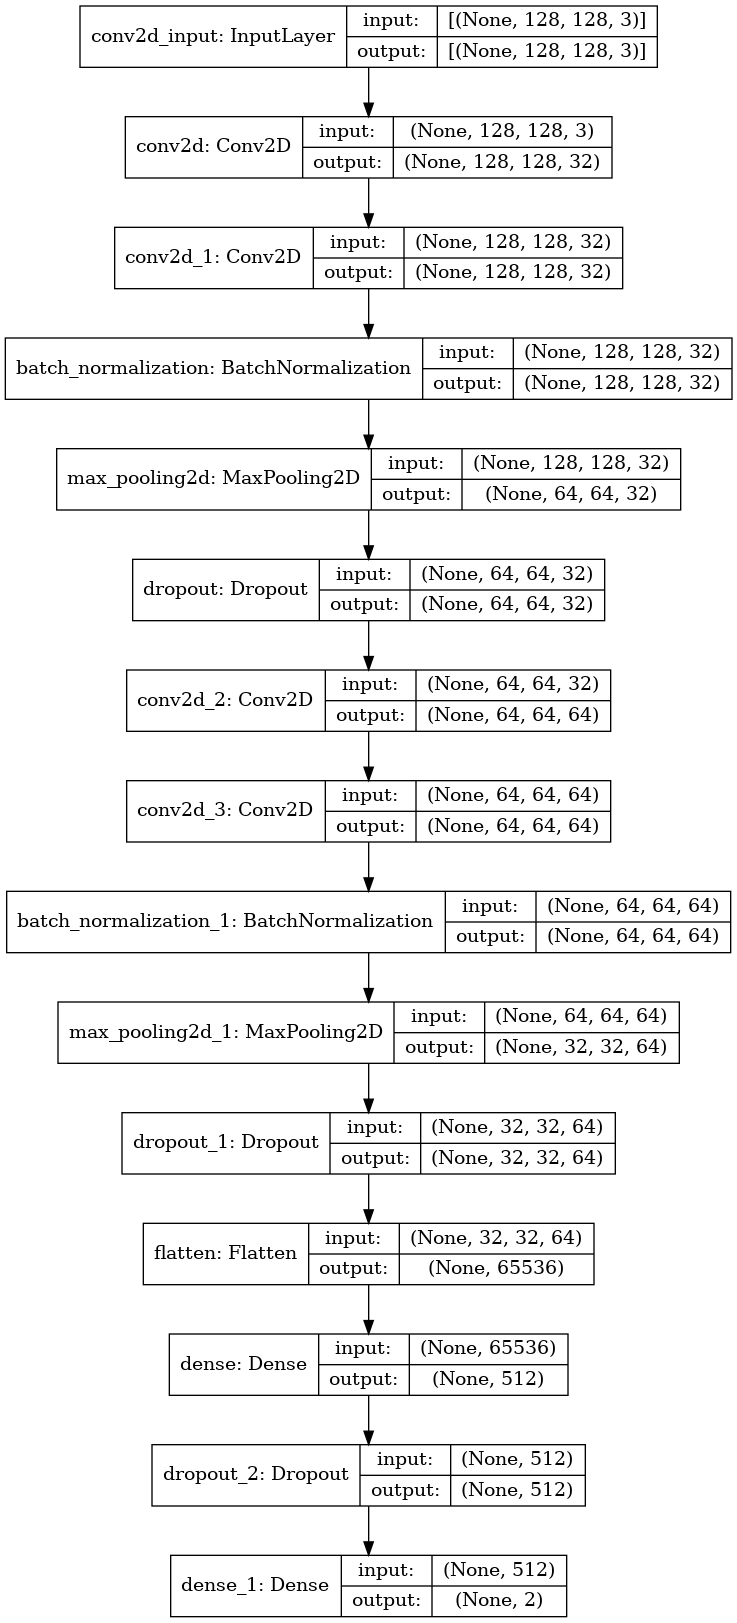
\includegraphics[scale=0.34]{Photos/model_plot.png}
\caption{Model Summary} \label{fig:model_plot}
\end{figure}

%%%%%%%%%%%%%%%%%%%%%%%%%%%%%%%%%%%%%%%%%%%%%%%%%%%%%%%%%%%%%%%%%%%%%%%%%%%%%%%%%%%%%%%%%%%%%%%%%%%%%%%%%%%%%%%%%%%%%%%%%%%%%%%%%%%%%%%%%%%%%%%%%%%%%%%%%%%%%%%%%%%%%%%%%%%%%%%%%%%%%%%%%%%%%%%%%%%%%%%%%%%%%%%%%%%%%%%%%%%%%%%%%%%%%%%%%%%%%

\section{Proposed Web Application}
This section explains about the Proposed Web Application. In this section detailed Algorithm, Flowchart and a Proposed layout is shown.
\subsection{Algorithm}
Step 1 : User is redirected to Login Page.\\
Step 2 : If the user is a New User. The Web App will redirect to Registration Page, else the user can login using his credentials. If login is unsuccessful redirect to Step 1.\\
Step 3 : After Login it will redirect to the Fact of the Day Page.\\
Step 4 : From the next page user will be able to select from 3 functionalities : Early Stage Detection, Traditional Procedures, Access History.\\
Step 5 : If user selects Early Stage Detection, webapp will redirect to the Detection Page. \\
Step 6 : User inputs Image.\\
Step 7 : System preprocesses the image.\\
Step 8 : This image is passed onto the preexisting Knowledge Base (Detection Model).\\
Step 9 : If tumour is detected, the system returns output as "Tumour Detected" and will intimate the authorities as well patient on an quick basis.\\
Step 10 : If tumour is not detected, the system returns output as "Tumour Not Detected" and will intimate the authorities as well patient on an quick basis.\\
Step 11 : If the user wants to access the menu again he can select the option and be redirected to Step 4.\\
Step 12 : If user selects Traditional Procedures, webapp will redriect to the Traditional Procedures Page.\\ 
Step 13 : If the user wants to access the menu again he can select the option and be redirected to Step 4.\\
Step 14 : If the user selects Access History, webapp will redirect to the Access History Page. \\
Step 15 : Access History Page will display the history of the patient if any. This data is directly linked to the Hospital's Database.\\
Step 16 : On clicking the About Us , Web App will redirect to the Meet Our Team Page.\\ 
Step 17 : On clicking Contact Us, Web App will redirect to Contact Us Page.\\ 
Step 18 : If user clicks Logout, Web App goes back to Step 1.\\

\subsection{Flowchart}
This is the detailed flowchart explaining the flow of the proposed webapp:
\begin{figure}[H]
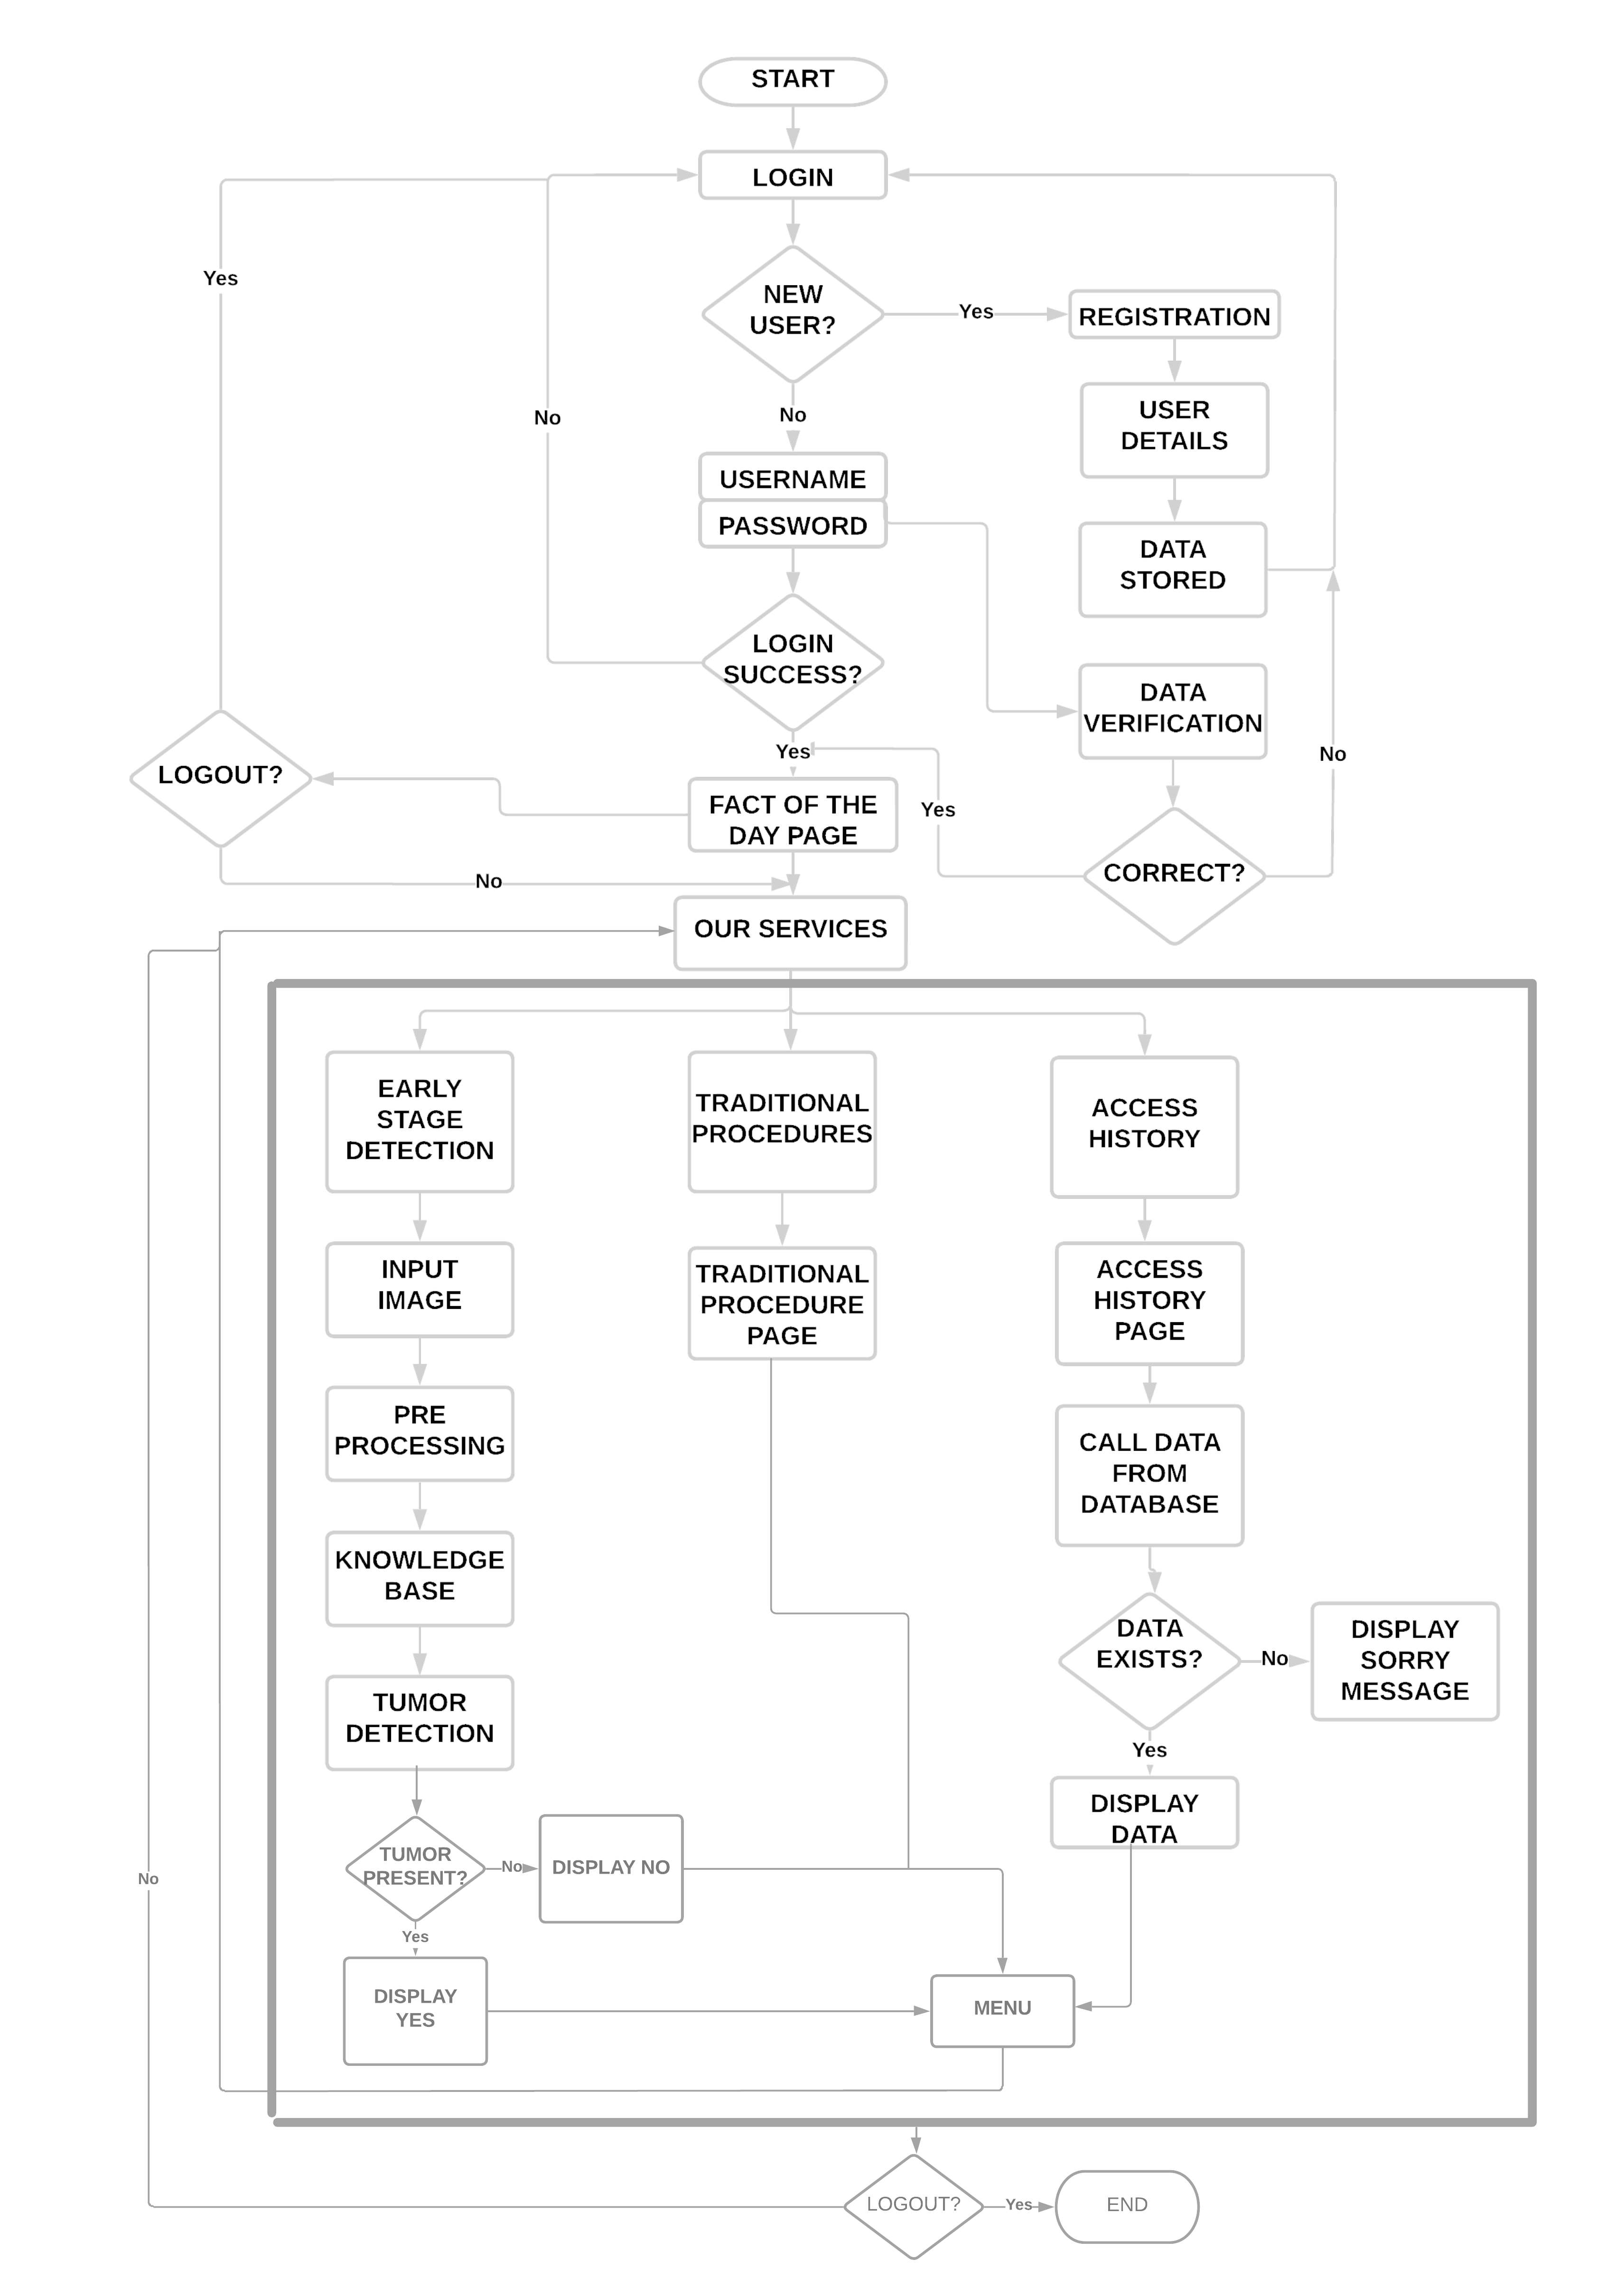
\includegraphics[scale=0.085]{Photos/webapp_flowchart.png}
\caption{Flowchart of the proposed Web Application} \label{fig:webapp_flowchart}
\end{figure}

\subsection{Proposed Web layout}
This section showcases the proposed web layout. This layout acts as a placeholder that will be used while developing the UI of the web application. While developing a web application, a layout development helps to understand the resources required, the colour schemes as well as to understand the routes of the application in consideration. \\ 
When the users will access the Web Application it will redirect to the login page \ref{fig:webapp_1} where both the Hospital Staff and the end user(Patient) will be able to login to access the webapp features.
\begin{figure}[H]
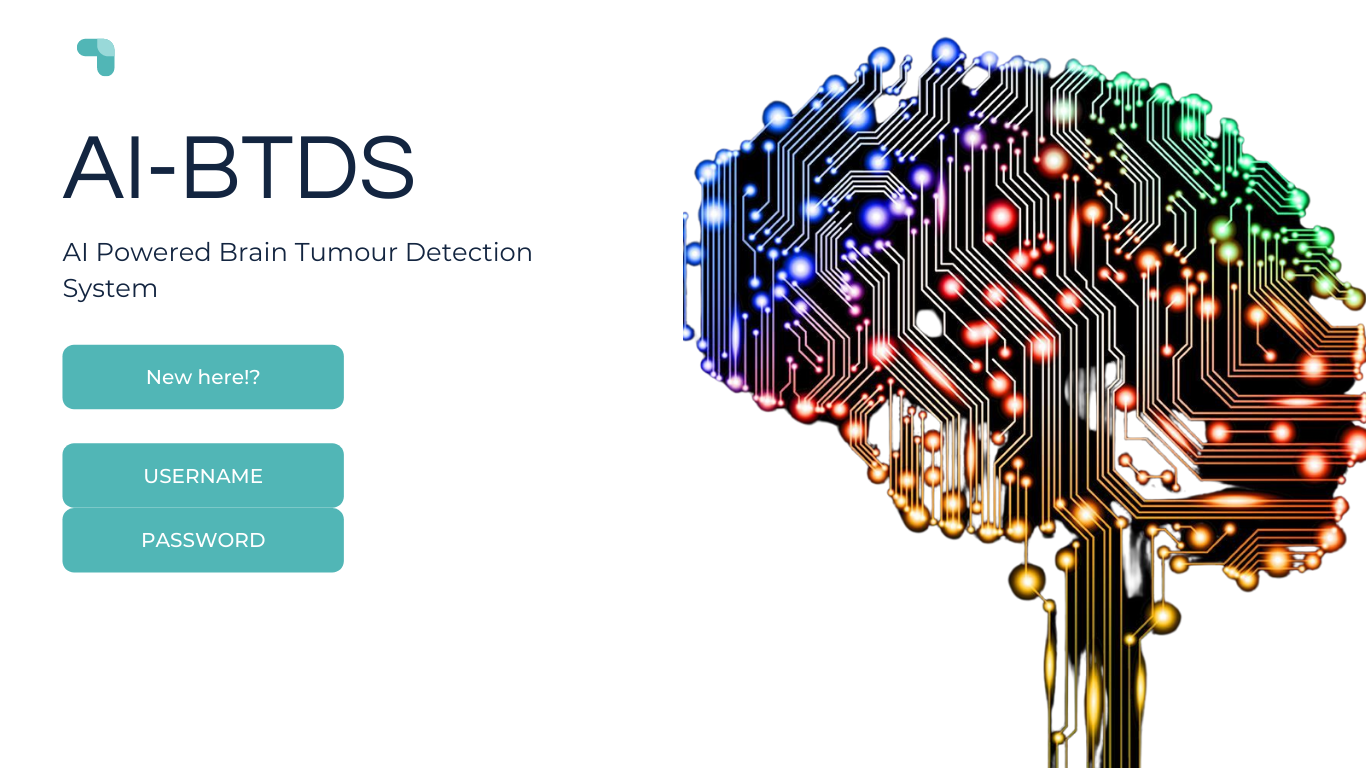
\includegraphics[scale=0.45]{Photos/webapp_1.png}
\caption{Login Page} \label{fig:webapp_1}
\end{figure}
The next figure is the Facts Page \ref{fig:webapp_2}. The web application will be having an additional functionality that will provide information on brain tumour as well so as to increase general awareness. This will be done using a random function generator that will display a new fact based on two factors, whether the user reloads the web page or based on time.
\begin{figure}[H]
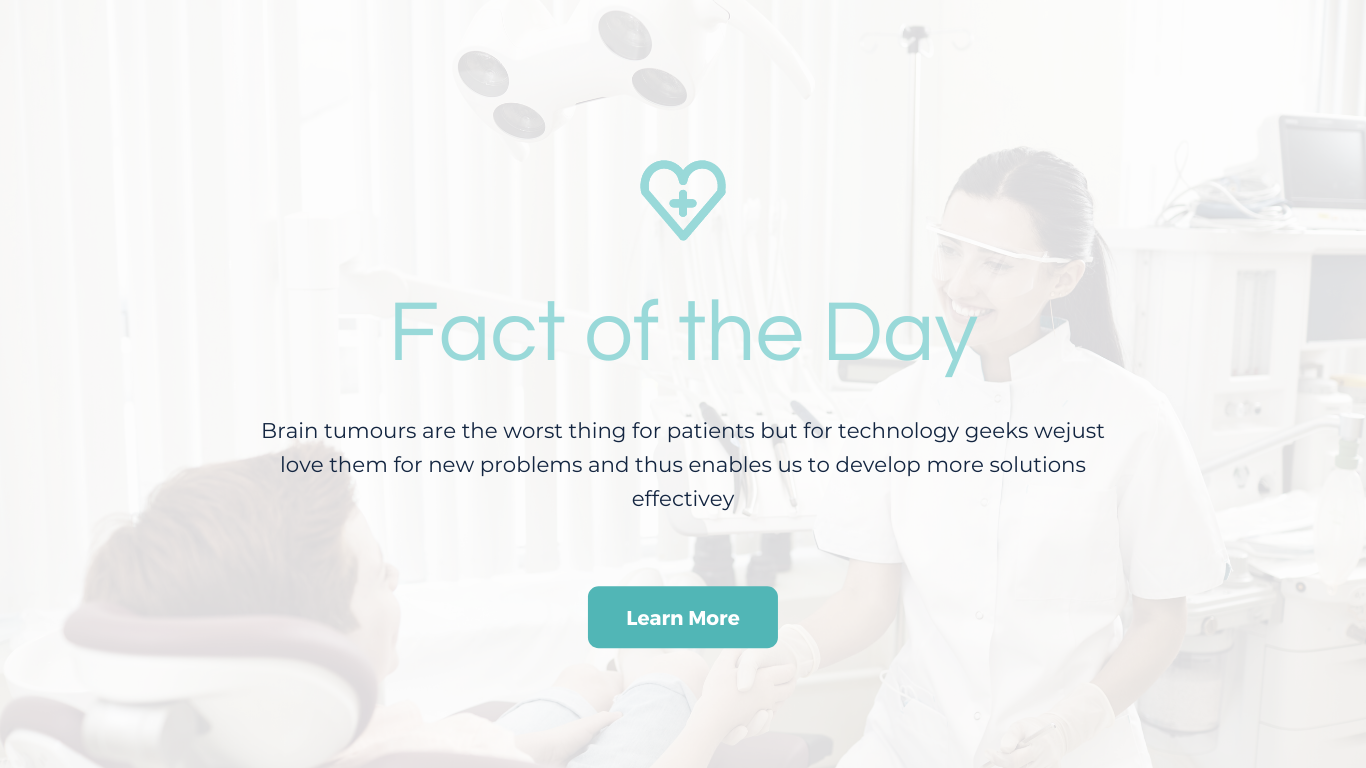
\includegraphics[scale=0.45]{Photos/webapp_2.png}
\caption{Fact of the Day} \label{fig:webapp_2}
\end{figure}
The next figure \ref{fig:webapp_3} refers to the "Our Services" page. Here the patients will be able to access any previous history if any as well as perform the actual Brain Tumour Detection. The traditional procedures tab will highlight about the traditional existing methods that are used in the detection procedure.
\begin{figure}[H]
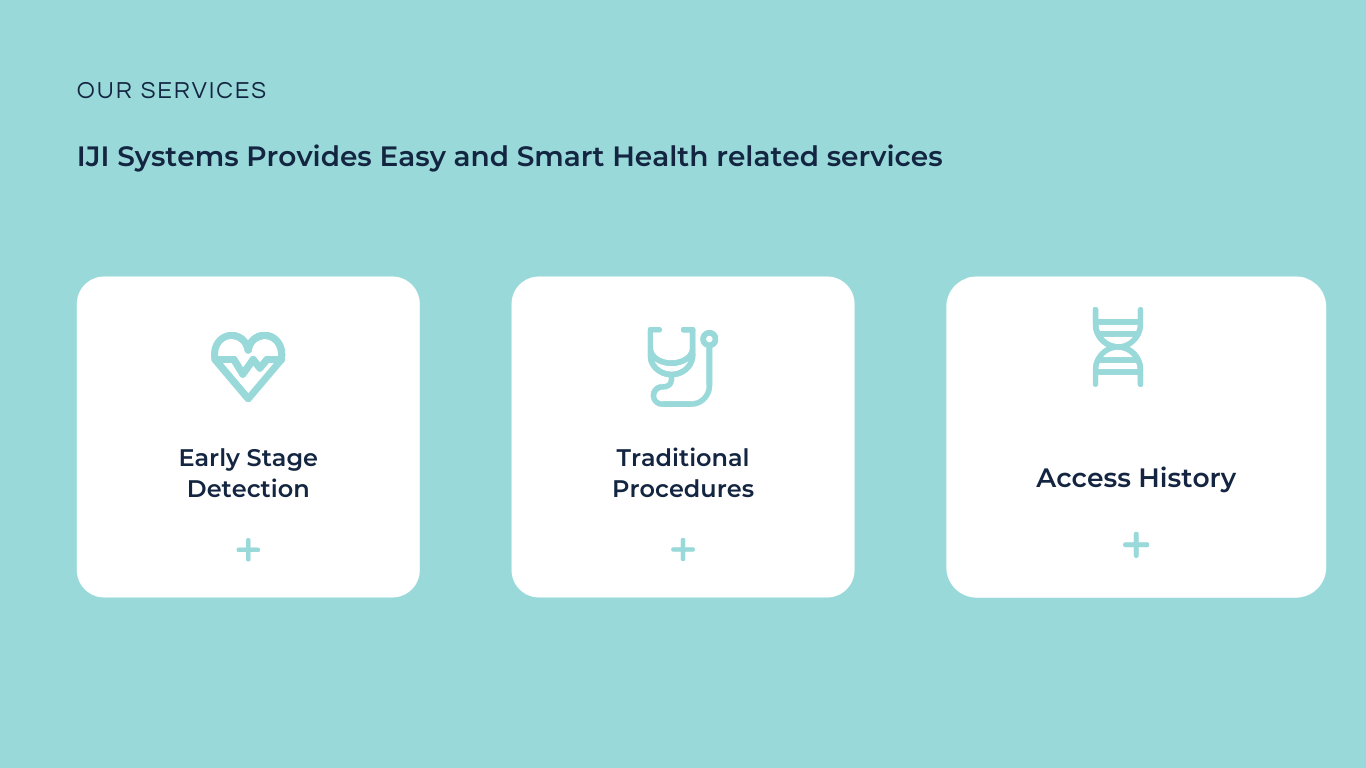
\includegraphics[scale=0.45]{Photos/webapp_3.png}
\caption{Page to Redirect to different functionalities} \label{fig:webapp_3}
\end{figure}
The figure \ref{fig:webapp_4} is the proposed Detection page. Here users will be able to upload the scanned MRI images. The system will then determine about Tumour and provide the results accordingly.
\begin{figure}[H]
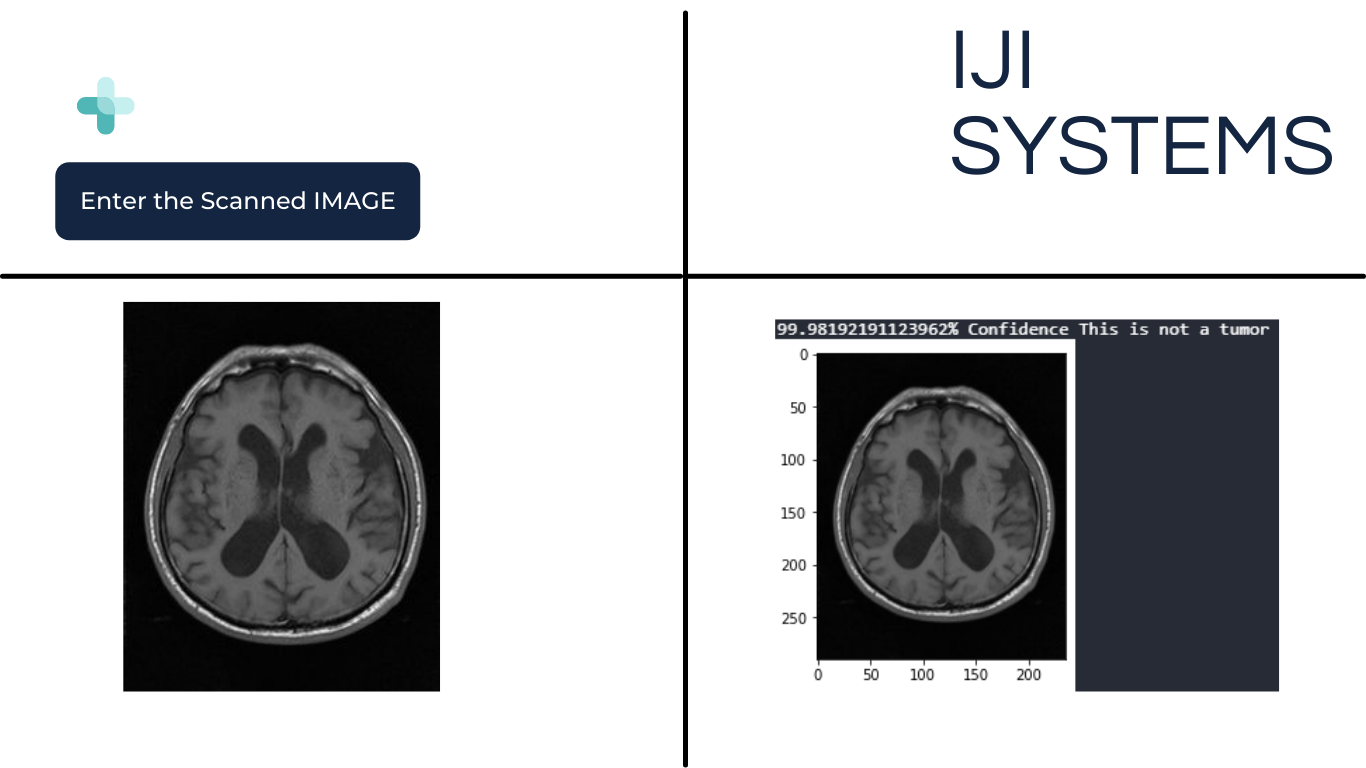
\includegraphics[scale=0.45]{Photos/webapp_4.png}
\caption{Brain Tumour Detection} \label{fig:webapp_4}
\end{figure}
Figure \ref{fig:webapp_5} highlights the team information page.
\begin{figure}[H]
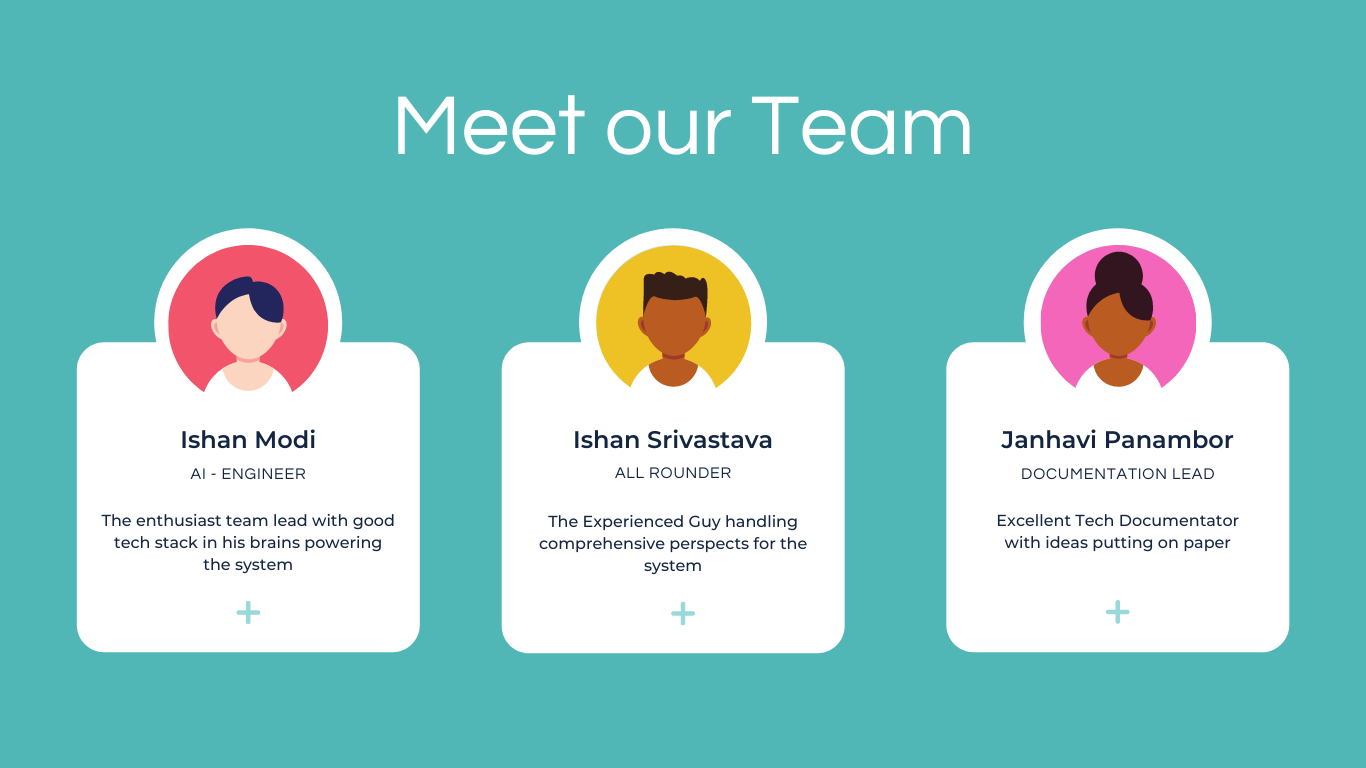
\includegraphics[scale=0.45]{Photos/webapp_5.png}
\caption{Team Information Page} \label{fig:webapp_5}
\end{figure}
Figure \ref{fig:webapp_6} highlights the Contact Us page.
\begin{figure}[H]

\includegraphics[scale=0.45]{Photos/webapp_6.png}
\caption{Contact Us Page} \label{fig:webapp_6}
\end{figure}